\section{Evaluation}

All images underwent the pipeline processing illustrated in Figure 
\ref{fig:pipeline} using the computational cluster at the University 
of Virginia.%
\footnote{
http://www.uvacse.virginia.edu/itc-clusters/
}  
Processing times varied approximately between 10--20 hours per subject
for the entire cortical thickness estimation procedure.  The propagation of the
NIREP labels to each subject using label fusion as described earlier
was performed in parallel and took approximately 60--90 hours per 
subject.  The scripts used to instantiate the processing jobs have all been made 
publicly available.
Average thickness values were tabulated per subject for each of the
32 NIREP labels.  Cerebral volumes for each subject derived from the brain 
extraction step were also calculated.  All these data were written to separate csv
files corresponding to data set (also included with the scripts) for subsequent 
analysis.

\subsection{Reproducibility}

\begin{table}
\centering
\begin{tabular*}{0.9\textwidth}{@{\extracolsep{\fill}} l c c}
\toprule
\multicolumn{1}{c}{Region} & \multicolumn{1}{c}{Left} & \multicolumn{1}{c}{Right} \\
\midrule
occipital & $5.36 \pm 6.92$ & $5.79 \pm 7.17$\\
cingulate & $3.7 \pm 4.49$ & $3.62 \pm 4.6$\\
insula & $4.52 \pm 4.27$ & $4.43 \pm 4.36$\\
temporal pole & $4.93 \pm 5.48$ & $4.81 \pm 5.01$\\
superior temporal & $4.74 \pm 5.34$ & $3.58 \pm 4.92$\\
infero temporal & $6.86 \pm 8.8$ & $6.58 \pm 9.21$\\
parahippocampal & $5.13 \pm 5.29$ & $4.61 \pm 3.76$\\
frontal pole & $7.1 \pm 8.07$ & $7.4 \pm 8.32$\\
superior frontal & $3.86 \pm 4.48$ & $3.85 \pm 4.31$\\
middle frontal & $6.58 \pm 7.8$ & $5.87 \pm 7.96$\\
inferior & $4.53 \pm 5.53$ & $4.26 \pm 5.49$\\
orbital frontal & $4.77 \pm 6.12$ & $5.39 \pm 5.36$\\
precentral & $4.46 \pm 4.5$ & $4.15 \pm 4.81$\\
superior parietal & $3.71 \pm 4.14$ & $3.67 \pm 3.78$\\
inferior parietal & $4.96 \pm 6.06$ & $4.96 \pm 6.74$\\
postcentral & $5.51 \pm 6.32$ & $6.02 \pm 6.01$ \\
\bottomrule
\end{tabular*}
\caption{Mean percent variability error ($\pm$ standard deviation) of repeated 
cortical measurements for both the Oasis and Kirby repeat scans
given for all 32 NIREP cortical labels (cf Table \ref{table:nirep_labels}).
These differences were not statistically significant (two-tailed $t$-test
with false discover rate (FDR) multiple comparisons correction).
}
\label{table:error}
\end{table}

Repeat scans of 40 subjects (20 Kirby subjects and 20 Oasis subjects) were 
used to determine the reproducibility of regional cortical thickness 
measurements. Similar to the assessment given in \cite{jovicich2013}, we
show regional reproducible thickness measurements, $T$, in terms of the
variability error:
\begin{align}
\varepsilon = \frac{|T_{scan} + T_{rescan}|}{0.5 \times (T_{scan} + T_{rescan})}
\end{align}
The error values for the 32 NIREP regions for both the Oasis and Kirby 
reproducibility data sets
are given in Table \ref{table:error}.  We also calculated the intraclass 
correlation coefficient 
(``ICC(2,1)'' in the notation of \cite{shrout1979}) to assess scan/rescan
reliability which showed reliable agreement ($ICC=0.95$).  

\subsection{BrainAGE Evaluation}


\begin{table}
\centering
\begin{tabular*}{0.9\textwidth}{@{\extracolsep{\fill}} l c c}
\toprule
\multicolumn{1}{c}{Analysis} & \multicolumn{1}{c}{$r$} & \multicolumn{1}{c}{mean error (years)} \\
\midrule
Gray matter probability & 0.93 & 6.17 \\  
Cortical thickness & 0.90 & 7.19 \\
\bottomrule
\end{tabular*}
\caption{Correlation and mean error values for both the gray matter probability and cortical thickness
{\it BrainAGE} evaluation.}
\label{table:brainAge}
\end{table}

\begin{figure*}
  \centering
  \begin{tabular}{cc}
  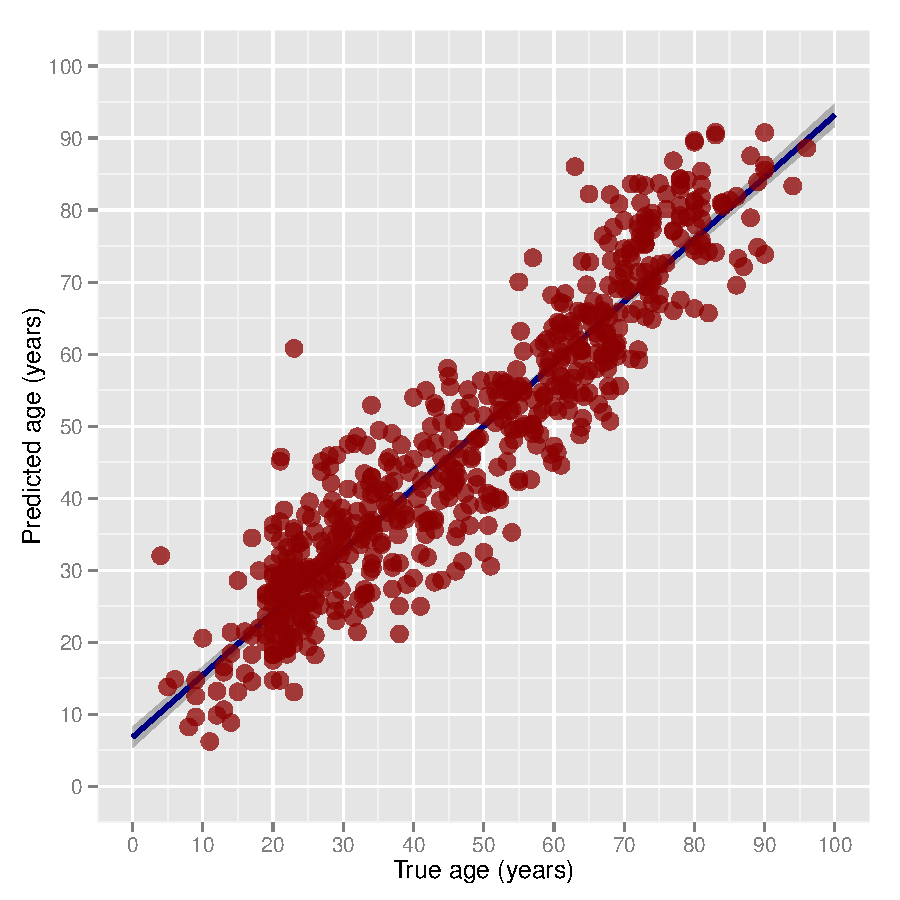
\includegraphics[width=65mm]{brainAgeBrainSegmentationPosteriors2.pdf} &
  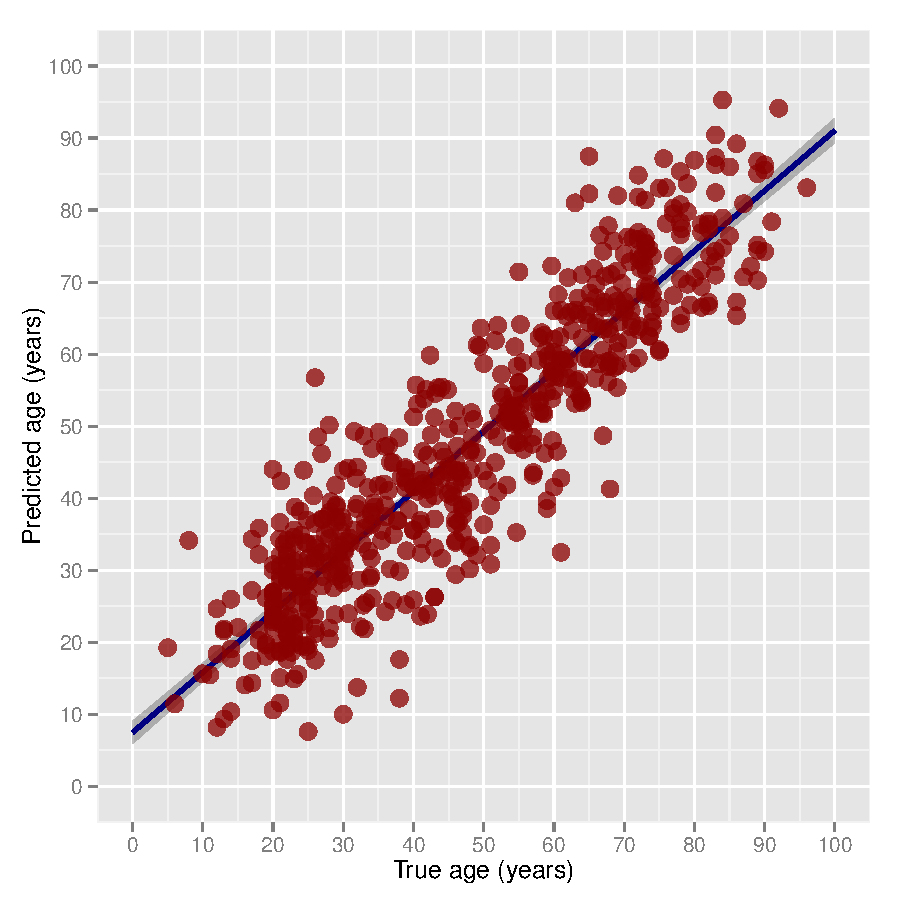
\includegraphics[width=65mm]{brainAgeCorticalThickness.pdf} \\
  (a) & (b) 
  \end{tabular}
  \caption{Results of RVM-based age prediction using (a) gray matter probability
  maps as in \cite{franke2010} and (b) cortical thickness maps both of which
  are derived from the previously described workflow.}
  \label{fig:brainAge}
\end{figure*}

In \cite{franke2010}, an estimation framework is presented for predicting 
apparent age from gray matter segmentation probability maps known as {\it BrainAGE}.  
Given a
normal age population spanning the age range of interest, the authors showed
how kernel regression methods can be used to reliably estimate age in a 
test group.  The basic processing pipeline includes 3-tissue segmentation
of a subject's T1, followed by registration to a common reference space (e.g.
the MNI template), and then smoothing (8 mm FWHM) and downsampling (8 mm 
isotropic resolution).  A principal components (PCA) model is constructed 
from the resulting aligned training image set.  The images of both the training set and 
testing set are decomposed into the bases of the PCA model which form the feature
set for relevance vector machine (RVM)-based learning and prediction, respectively. 

We applied the BrainAGE framework to the gray matter probability maps derived
from our pipeline.  We also applied the same strategy to predicting age from 
our cortical thickness images.  We randomly separated the images of each of the 
four cohorts into approximately two equal subgroups (testing and training).
Construction of the PCA model and decomposition of all images into the corresponding 
bases were performed on the training group using tools developed from the Insight Toolkit.%
\footnote{
http://www.itk.org/Doxygen/html/classitk\_1\_1ImagePCADecompositionCalculator.html  
}
We used R%
\footnote{
http://rss.acs.unt.edu/Rdoc/library/kernlab/html/rvm.html
} 
to train the RVM model, perform prediction, and plot the results for both
analyses (shown in Fig. \ref{fig:brainAge}, cf. Fig. 3 in \cite{franke2010}).
Again, testing and training data, as well as R scripts used to produce the 
plots in Fig. 3 are publicly available.  
The resulting predictions for both image sets are quite similar as demonstrated 
visually in Fig. 3.  The correlation coefficients and mean errors in Table 
\ref{table:brainAge} between the
two approaches are also evidence of mutual corroboration.

\subsection{Gender Structural Connectivity Across Age Using Cortical Thickness}
As mentioned in the Introduction, cortical thickness has
been used to determine structural connectivity relationships 
where strong correlations in regional cortical 
thickness values across subjects provide evidence for anatomical
connectivity \citep{he2007,chen2008,he2008}.
We use the compiled cortical thickness data to demonstrate the longitudinal
variation in gender-based differences in structural connectivity.




\begin{figure*}
  \centering
  \begin{tabular}{c}
  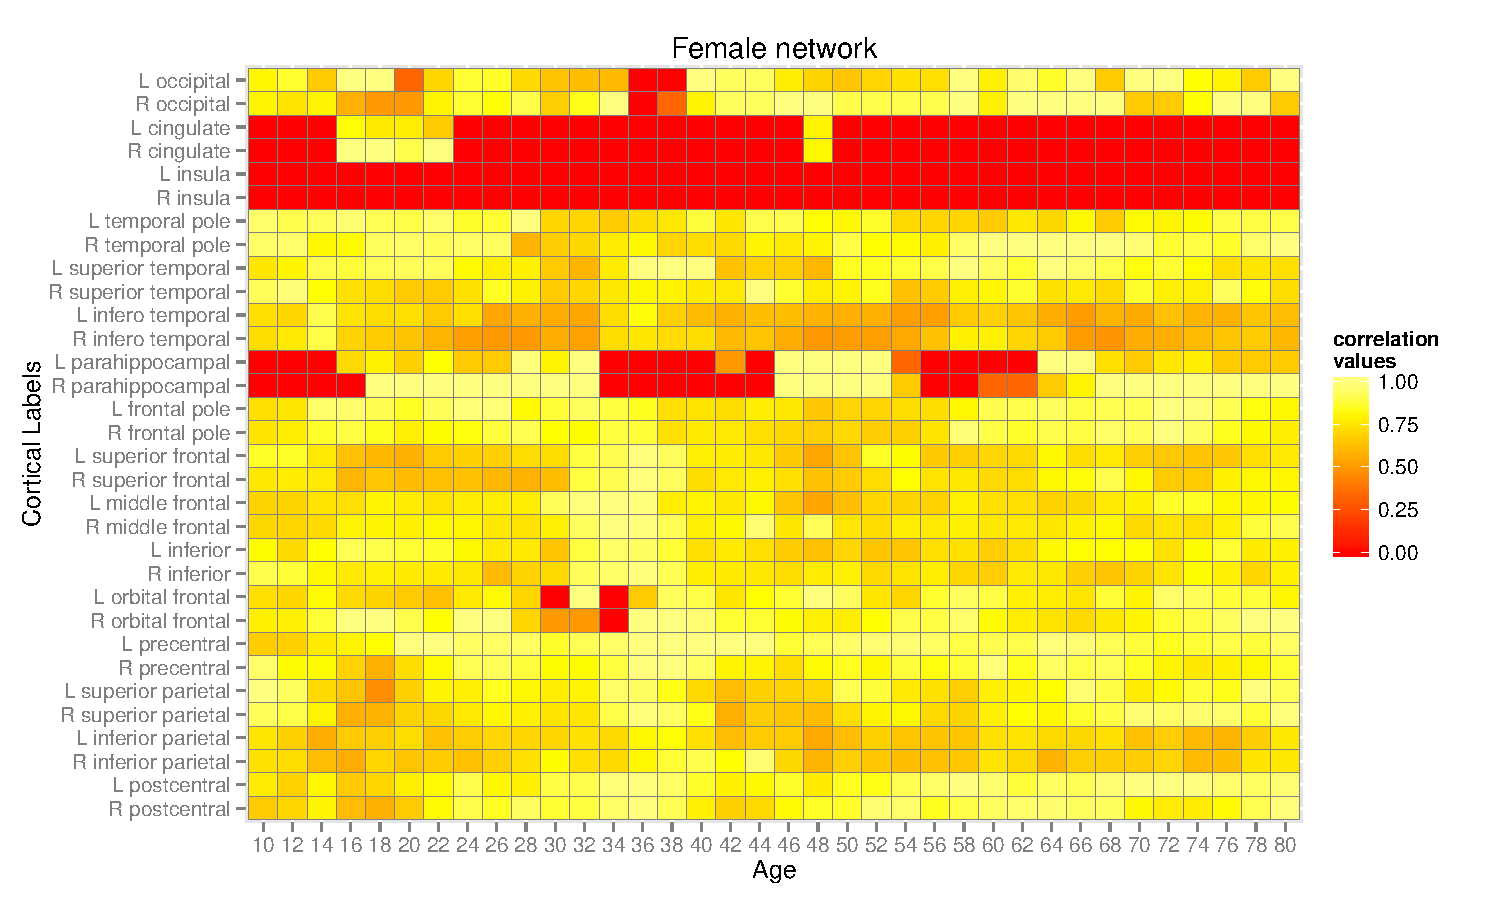
\includegraphics[width=140mm]{femaleNetwork.pdf} \\
  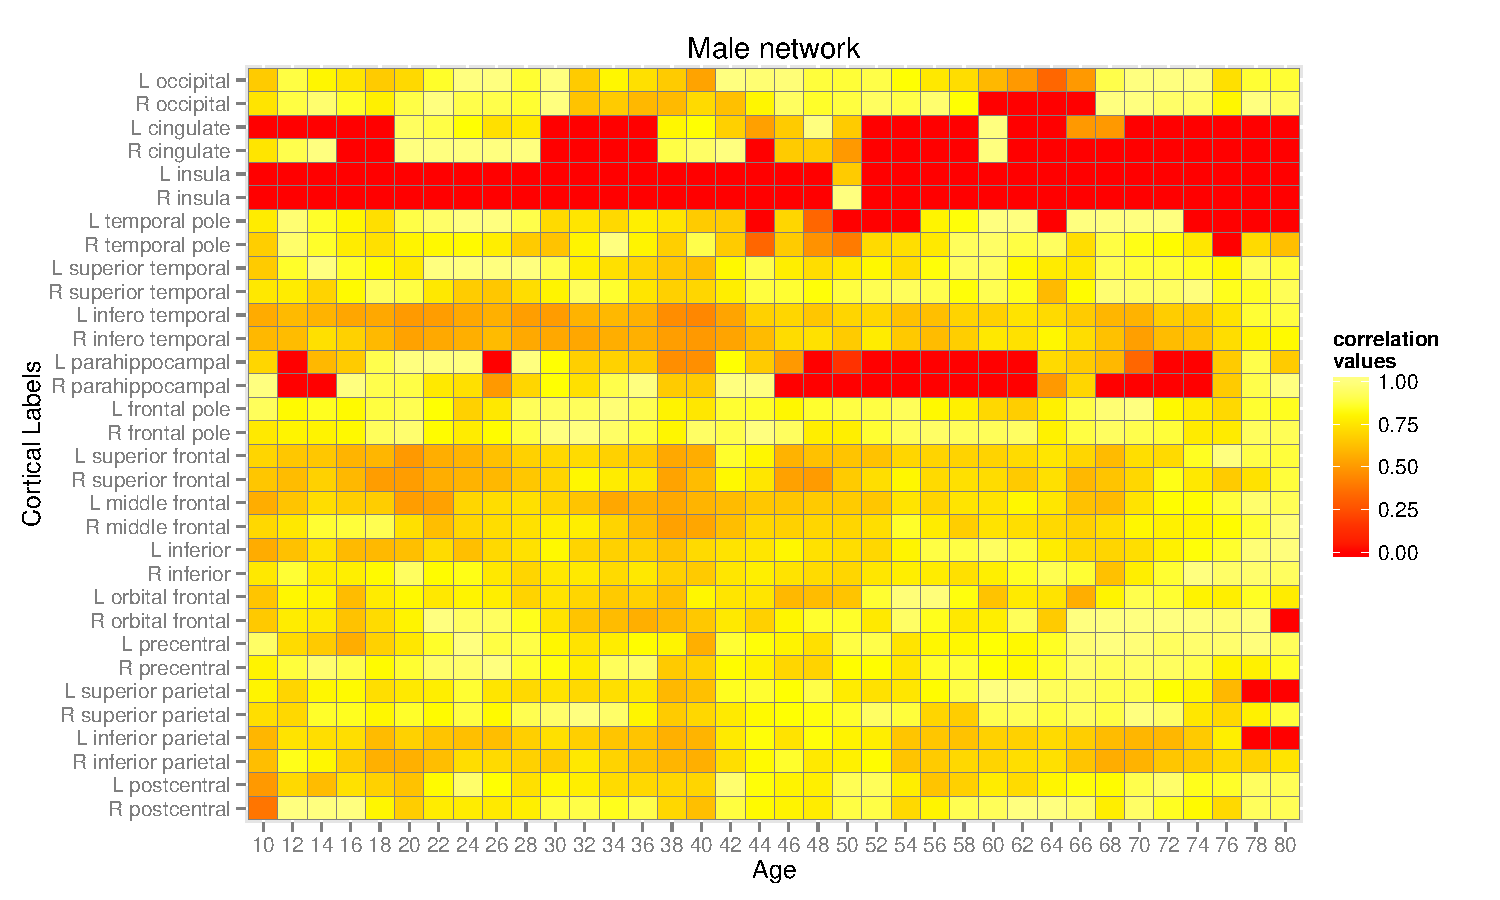
\includegraphics[width=140mm]{maleNetwork.pdf}
  \end{tabular}
  \caption{Transitivity (clustering coefficient) values across age for both the female (top)
  and male (bottom) networks.  The transitivity at a given spatio-temporal
  location in the heat map describes the probability that the specified 
  vertex is connected to adjacent vertices.  Thus, higher probability values indicate a
  greater structural connectivity.
  }
  \label{fig:network}
\end{figure*}

